%!TEX root = ../../main.tex

\chapter{Quality of Nanodiamonds}	\label{ch::crystal_quality}
\chaptermark{Quality}

		\begin{remark}
				Ich hab das kapitel jetzt nochmal ueberarbeitet indem ich den aufbau vom SiV papier hier uebernommen hab. Das gibt nochmal einen besseren ueberblick. Es gibt aber noch loecher die du nochmal dezidiert stopfen solltest. Besonders die section mit den post-processing methoden ist noch nicht auf dem niveau der anderen sections in dem kapitel.

				\begin{itemize}
					\item In der introduction werden qualitaetsprobleme genannt und ein paar methoden die da helfen sollen. Hier muss noch kurz erwaehnt werden warum die methoden helfen.
					\item In der ersten section sind annealing und oxidation zusammen. Im text steht aber nur was annealing oder? Falls oxidation dann erst in der naechsten section kommt, sollte man die ueberschriften aendern. Ich kenn mich halt nicht aus, d.h. das passt noch nicht. Es muss auch klar werden welche probleme diese methoden potentiell loesen und warum.
					\item Was die surface treatments bewirken sollen bzw. wie die die qualitaetsprobleme minimieren? Da ist auch von shells die rede und ich hab keine ahnung was das fuer dinger sind. Hier fehlt auch noch was.
					\item Wenns um \TEM messungen geht, dann ist hier auch von \nd boundaries die rede. Hier sollte jetzt auch eine diskussion boundaries einfliessen, bzw. was fuer negative effekte die haben koennen.
				\end{itemize}

		\end{remark}

		In this thesis we perform measurements of single \sivs in wet-milled \nds. To this end, we require high quality diamond nanoparticles containing a single \siv each. In this context we use the term quality as a measure of how close diamond crystals are to their pristine form. The presence of lattice imperfections such as additional vacancies, lattice strain, impurities or the inclusion of graphite or amorphous carbon is known to adversely affect crystal quality \cite{Zaitsev2001,Prawer2004,Orwa2000}.

		Surface contamination like graphite and amorphous $sp^2$ hybridized carbon atoms manifest themselves as additional peaks in the Raman spectrum.
		Strain in the diamond lattice broadens the first order Raman peak and causes it to shift to higher or smaller wavenumbers.
		Similarly, high concentrations of lattice defects cause additional peaks, a broadening of the first order Raman peak and a shift towards smaller wavenumbers.

		To improve crystal quality and to reduce the mentioned distracting effects the following methods are depoyed here: Annealing in a vaccuum, oxidation in air as well as surface treatments involving plasmas\todo[fancyline]{Hier fehlt jeweils ein kurzer satz was die dinger bewirken sollen.}.

		To study the effectiveness of these treatments and to gauge the quality of our \nd samples we rely on Raman spectroscopy and TEM imaging. The former is used to detect strain, quantify defect concentration and the presence of carbon in non-diamond phases, while the latter enables imaging of individual \nds revealing details in crystallinity such as crystal boundaries.

		\section{Quality-improving Post-Processing Treatments}

			\subsection{Annealing and Oxidation}\label{subsection::ann_ox}

				During \si implantation the diamond lattice gets damaged by the penetrating ions.
				sp$^2$ bonds, carbon interstitials and vacancies disrupt the metastable equilibrium of the diamond phase. Hence, there is a tendency for damaged diamond to "tip over" to the thermodynamically stable form of carbon, i.e. graphite.
				At temperatures above about \SI{500}{\celsius}, vacancies in the diamond lattice become mobile and diffuse towards the surface\cite{Dresselhaus1992}.
				Literature suggests, that annealing at \SI{900}{\celsius} for \SI{1}{\hour} is sufficient to remove most of the damage following implantations, that however some damage remains even after annealing at \SI{900}{\celsius} for \SI{1}{\hour}.
				To reduce the damage in the diamond lattice, we anneal the implanted diamonds at \SIrange{900}{1200}{\celsius} for \SIrange{3}{6}{h} in vacuum (\SI{e-6}{Pa}).
				\\
				The surface of the \nds is contaminated with graphite and amorphous sp$^2$ hybridized carbon \todo[fancyline]{warum}.
				The vacancies which diffuse towards the surface during annealing further increase the amorphous carbon content on the surface of the \nds \cite{}.
				We apply oxidation in an oven under ambient air at a temperature of \SI{450}{\celsius} for \SIrange{3}{6}{h}.

			\subsection{Surface Treatment With Gas And Plasma}\label{subsection::plasma}

				% Cardiff
				We wanted to know wether surface treatment with different gasses had an influence on the emission properties, so we treated them with hydrogen (\ch{H2}), oxygen (\ch{O2}), ozone (\ch{O3}) all both at room temperature and at \SI{500}{\celsius}; and also with \ch{H2} plasma.
				However, we found that most \nds treated in this way only showed luminescence which immediatly bleached when illuminated with a cw \SI{660}{nm} laser even at low excitation powers of \SI{200}{\micro\watt}, or no luminescence at all.
				We double-checked with a CCD-image of the surface to be sure that there are \nds in the focus.
				This bleaching occured so quickly, that after a scanning no spectrum could be taken.
				The only samples which did yield spectra with measureable \ZPLs were the ones treated with \ch{H2}.
				However, also these \sivs were not single ones.
				Therefore, we did not further investigate these samples.
				\\
				% C-Schalen
				One sample showed shells around the \nd after oxidizing in air.
				We attribute this effect to a contamination in the oven.
				When we illuminated these \nds in the SEM for several moments, the shell went away.
				We therefore deducted that the shell is organic material.
				To get rid of the shells on the whole sample, we treated it with oxygen-argon plasma for \SI{3}{min}\footnote{Treatment performed by \schmauch}.
				After the first treatment, the shells were smaller, but not gone.
				So we put them into the oxygen-argon plasma again for \SI{3}{min}, however, the shells were bigger than before any treatment.
				We tried another approach to get rid of the shells with ozon treatment for \SI{4}{\hour} at \SI{360}{\celsius}.
				Before ozon treatment there the diamond Raman line and other Raman lines visible.
				After surface treatement, more lines appeared and all of these other lines got more intense.
				There are probably organic contaminations on the sample in which functional groups got introduced by the ozon treatment.
				We did not further investige this sample and defined it as broken.

		\section{Raman Measurements}

			Raman spectroscopy of various samples gives insight to crystal quality and surface contamination of \nds.
			Raman scattering is the inelastic scattering of a photon $\hbar\omega_i$ on a molecule or crystal lattice in the initial state $\ket{i}$ with energy $E_i$.
			The molecule of cristal transitions into a higher energy state $E_f$ and the scattered photon with frequency $\omega_s$ looses the energy $\Delta E = E_f - E_i = \hbar(\omega_i-\omega_s)$.
			Therefore, energy is exchanged between the photon and the excited matter, changing the rotational or oscillation energy of the involved molecule or the oscillation energy, i.e.\ phonons of the crystal lattice.
			The Raman shift is typically referenced in wavenumbers.
			It is given by:

			\begin{equation}
				\Delta \omega = \left( \frac{1}{\lambda_{ex}}-\frac{1}{\lambda_R}\right)
			\end{equation}

			As every solid exhibits characteristic phonon modes tied to the properties of its lattice structure, Raman spectroscpy can be used to characterize diamond.
			Raman measurements of wet-milled \nds give insight into the issues of surface contamination, lattice strain and defect concentration:
			Surface contamination like graphite and amorphous sp$^2$ hybridized carbon atoms cause additional peaks in the Raman spectrum.
			A high defect concentration may lead to additional peaks, a broadening of the first order Raman peak and a shift to smaller wavenumbers.
			Strain in the diamond broadens the first order Raman peak and causes a shift to higher wavenumbers \cite{Zaitsev2001,Prawer2004,Orwa2000}.
			\\
			For the Raman measurements the same layout of the setup described in \autoref{ch::confocal_setup} is used.
			As excitation lightsource, a \SI{532}{nm} continuous wave diode laser is used (IO \todo[fancyline]{type}).
			It provides single frequency mode laser light, a prerequisite for Raman investigations.
			The beamsplitter is a dichroic mirror (DRLP645), the laser light is additionally filtered out with a $532$ Notch filter in the detection path in front of the single mode fiber instead of a longpass filter.
			With these adaptions, the combination of the confocal unit and the spectrometer serves as a Raman spectrometer.
			As the diamond Raman line is very narrow, the \SI[per-mode=symbol]{600}{\lines\per\mm} grating is used to as a starting point. Detailed measurements are realized using \SI[per-mode=symbol]{1200}{\lines\per\mm} and \SI[per-mode=symbol]{1800}{\lines\per\mm} gratings.
			\\

			% Versuchsdurchfuehrung
			Since the size of single \nds is on the order of tens of nanometers, low signal intensities can become an issue when taking Raman measurements.
			To overcome this problem we persue two different approaches:
			\begin{enumerate}[label=\alph*),ref=\alph*)]
				\item \Nd Clusters: \label{item::raman_gband} Collective measurements are carried out at several areas on the sample \insituS. Since this sample is densely covered with \nds, collective measurements of clusters of \nds (\cref{subfig::raman_no}) achieves higher signal intensities.
				\item Big \Nds: \label{item::raman_implanted} Raman measurements are carried out on the implanted sample \implantedTao. For this sample, diamond particles are big enough to yield sufficient intensities on single \nds.
			\end{enumerate}

			\begin{figure}
				\begin{subfigure}[htp]{0.45\linewidth}
					\centering
					\testbox{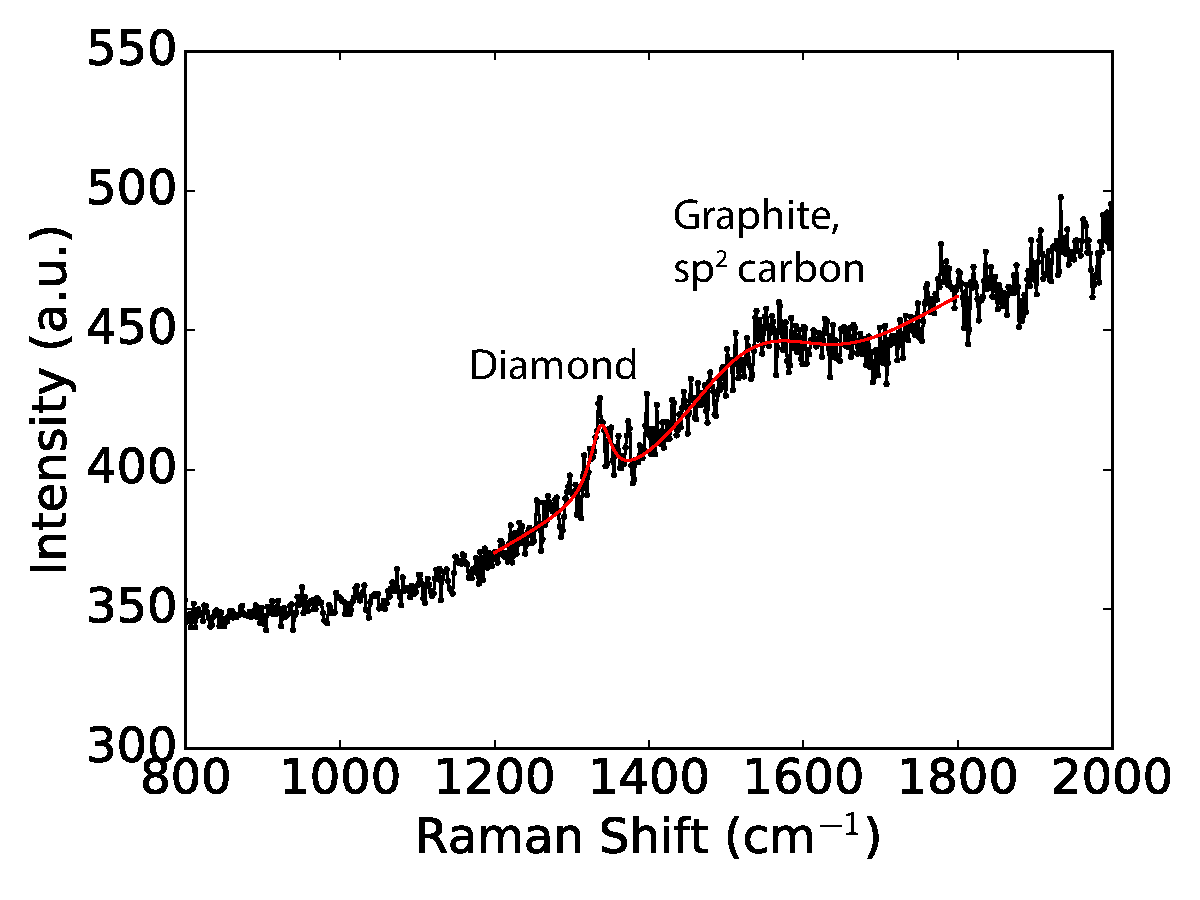
\includegraphics[trim = 0 0 0 0 , clip = true, width = \linewidth]{./pics/Ir25_spectrum_scan_xy-05x6y8_4000uW_t60_wavenumber_fit.pdf}}
					\caption{}\label{subfig::raman_no}
				\end{subfigure}
				\hfill
				\begin{subfigure}[tp]{0.45\linewidth}
					\centering
					\testbox{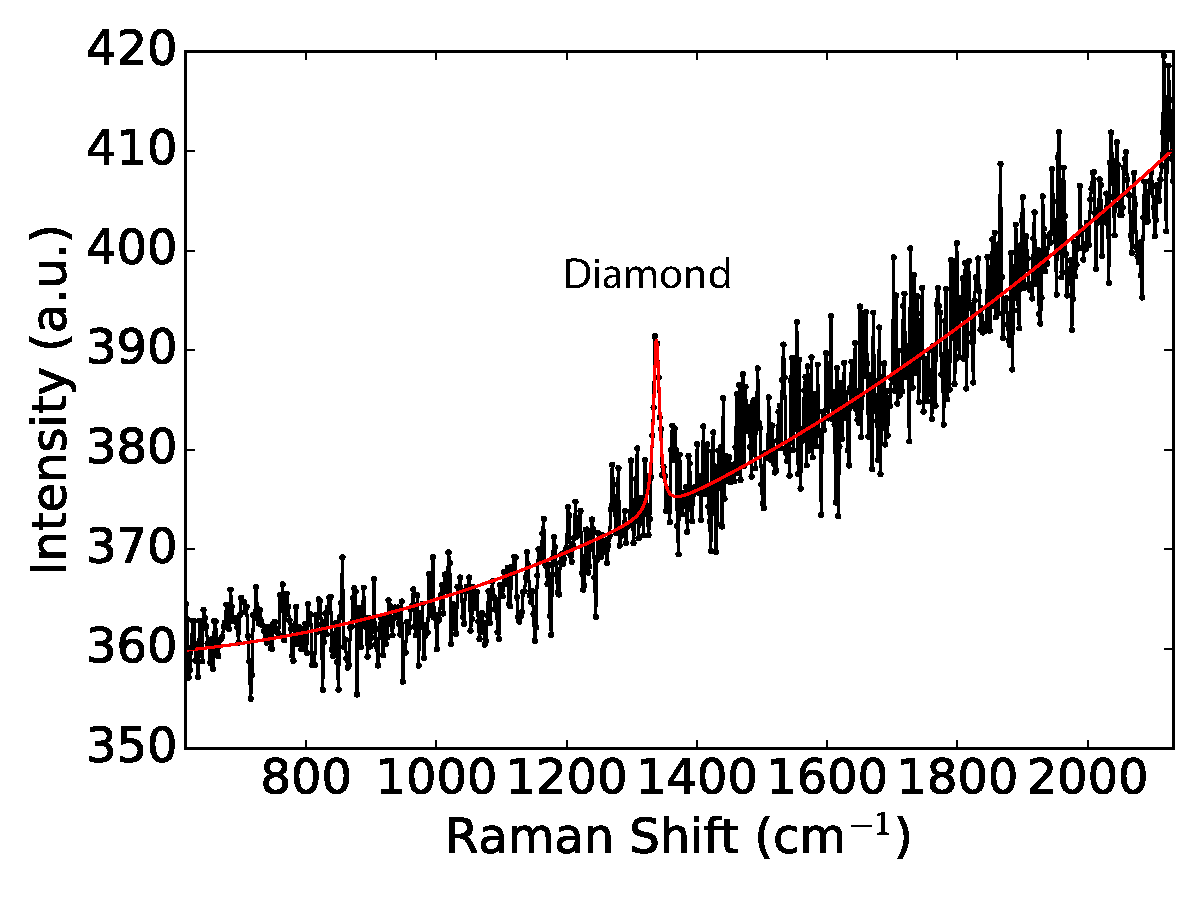
\includegraphics[trim = 0 0 0 0,  clip = true, width = \linewidth]{./pics/Ir_22_spe_scan_xy-02x7y7_550-600nm_t240_wavenumber_fit.pdf}}
					\caption{}\label{subfig::raman_ox}
				\end{subfigure}
				\caption[Raman spectrum of a single \nd]{Raman measurements, black: data, red: fit. (a) Raman measurement before oxidation, sample \insituS. The diamond Raman peak is situated at \SI{1338}{\per\centi\meter}. The broad feature around \SI{1580}{\per\centi\meter} corresponds to the graphite G-band. (b) Raman measurement after oxidation, sample \insituSo. The G-band has vanished, indicating removal of graphite and amorphous sp$^2$ hybridized carbon.}
				\label{fig::raman}
			\end{figure}

			\subsection{Surface Contamination}\label{subsection::raman_surface_contamination}
				We test the impact of oxidation treatment as described in \cref{sec::methods} on surface contamination.
				\cref{subfig::raman_no} shows a measured Raman spectrum of a sample without oxidation treatment (\insituSn).
				To verify reproducibility, the measurement is performed on three different spots of the sample.
				The narrow peak in \cref{subfig::raman_no} corresponds to the first order diamond Raman peak and will be further analyzed in \cref{subsection::raman_strain}.
				The spectrum also shows a broad peak with a Raman shift of about \SI[separate-uncertainty]{1582+-5}{\per\centi\meter}.
				This shift corresponds to the G-band due to amorphous sp$^2$ hybridized carbon atoms and graphite.
				The exact G-band position and \lw is sensitive to parameters such as the clustering of the sp$^2$ phase, bond-length and bond-angle disorder, presence of sp$^2$ rings or chains, and the sp$^2$/sp$^3$ ratio \cite{Ferrari2004}.
				The \nd Raman spectra are considerably modified after \ox in air at \SI{450}{\degreeCelsius}.
				To verify this, we perform Raman measurements on three different spots of a sample produced in the same process as the above mentioned, which is additionally oxidized (\insituSo).
				While the G-band peak is present in every measurement performed on a non-oxidized sample, it is not present in any of the oxidized samples (\cref{subfig::raman_ox}), indicating successful removal of sp$^2$ hybridized carbon and surface graphite.

			\subsection{Defect Concentration}\label{subsection::raman_defect_concentration}
				Several effects impact the first order diamond Raman line:
				\begin{enumerate*}
					\item defects in the diamond lattice,
					\item hydrostatic pressure,
					\item uniaxial or more complicated stress configurations.
				\end{enumerate*}
				In the measurement on \nd clusters the width of the diamond Raman peak of sample \insituS varies between \SIlist{15; 30}{\per\centi\meter} without \ox treatment, but is only \SIrange{9}{11}{\per\centi\meter} after the \ox process.
				A possible reason for this change of the width is improved crystal quality \cite{Prawer2004}.
				In the measurement on big \nds we measured a Raman line at \SI[separate-uncertainty]{1308+-5}{\per\centi\meter} (denoted line R1) which exhibits a broad \lw of \SI[separate-uncertainty]{25+-5}{\per\centi\meter}.
				One plausible explanation for both the position and the \lw of the Raman line are defects in the diamond lattice\cite{Prawer2004}.

			\subsection{Lattice Strain}\label{subsection::raman_strain}

				We investigated how strain in the diamond lattice manifests itself in both measurements on \nd clusters and on big \nds.
				In the Raman measurement on \nd clusters, the position of the diamond Raman peak is the same for oxidized (\insituSo) and non-oxidized (\insituSn) samples, indicating that oxidation does not affect strain in the diamond.
				However, the Raman shift of both non-oxidized and oxidized samples amounts to \SI[separate-uncertainty]{1338+-5}{\per\centi\meter}, as compared to the literature value of \SI{1332.5}{\per\centi\meter} of pristine diamond \cite{Zaitsev2001} (given uncertainties are governed by spectrometer resolution).
				This shift indicates the presence of strain in the diamond particles.
				\\
				Performing the Raman measurement on big \nds we found one diamond Raman line at \SI[separate-uncertainty]{1308+-5}{\per\centi\meter} (line R1), one at \SI[separate-uncertainty]{1345+-5}{\per\centi\meter} (line R2) and one at \SI[separate-uncertainty]{1348+-5}{\per\centi\meter} (line R3), indicating a broad distribution of strain among the individual diamond particles (uncertainties governed by spectrometer resolution).
				Only line R1 can be explained with a high defect concentration in the diamond lattice due to its shift to smaller wavelenths.
				However, a more consistent model which explains all occurring shifts is the presence of strain in the diamond nanoparticles.
				From the \lws in the measurement on big \nds, the strain in the diamond is calculated using the equation for hydrostatic pressure \cite{Prawer2004}
				\begin{equation}
					\omega(P)=\omega_0+a_1P+a_2P^2,
				\end{equation}
				where $\omega_0=\SI{1332.5}{\per\centi\meter}$, $a_1=\SI{2.83}{\per\centi\meter\per\giga\pascal}$ and $a_2=\SI{-3.65e-3}{\per\centi\meter\per\giga\pascal}$.
				The calculation yields a pressure in the investigated diamonds of \SI{-8.56}{\giga\pascal} tensile stress and \SIlist{4.26;5.50}{\giga\pascal} compressive stress.
				Pressure uncertainties due to the Raman line measurements are smaller than one Pascal and are therefore neglected.
				Under hydrostatic pressure, the triply degenerate first order Raman peak remains degenerate, while under uniaxial and more complex stress configurations (biaxial stress, shear stress etc.) mode splitting occurs \cite{Prawer2004}.
				As mentioned above, we observe broad \lws up to \SI[separate-uncertainty]{25+-5}{\per\centi\meter}.
				The broad \lws of the Raman lines may be attributed to uniaxial strain, as mode splitting manifests itself in a broadening of the peak due to limited spectrometer resolution.
				Therefore, we conclude that both hydrostatic and uniaxial strain is present in the \nds.

		\section{Transmission Electron Spectroscopy Measurements}{\label{sec::tem}}

			\begin{figure}[htp]
				\begin{subfigure}[t]{ 0.49\linewidth}
					\centering
					\caption{}
					\testbox{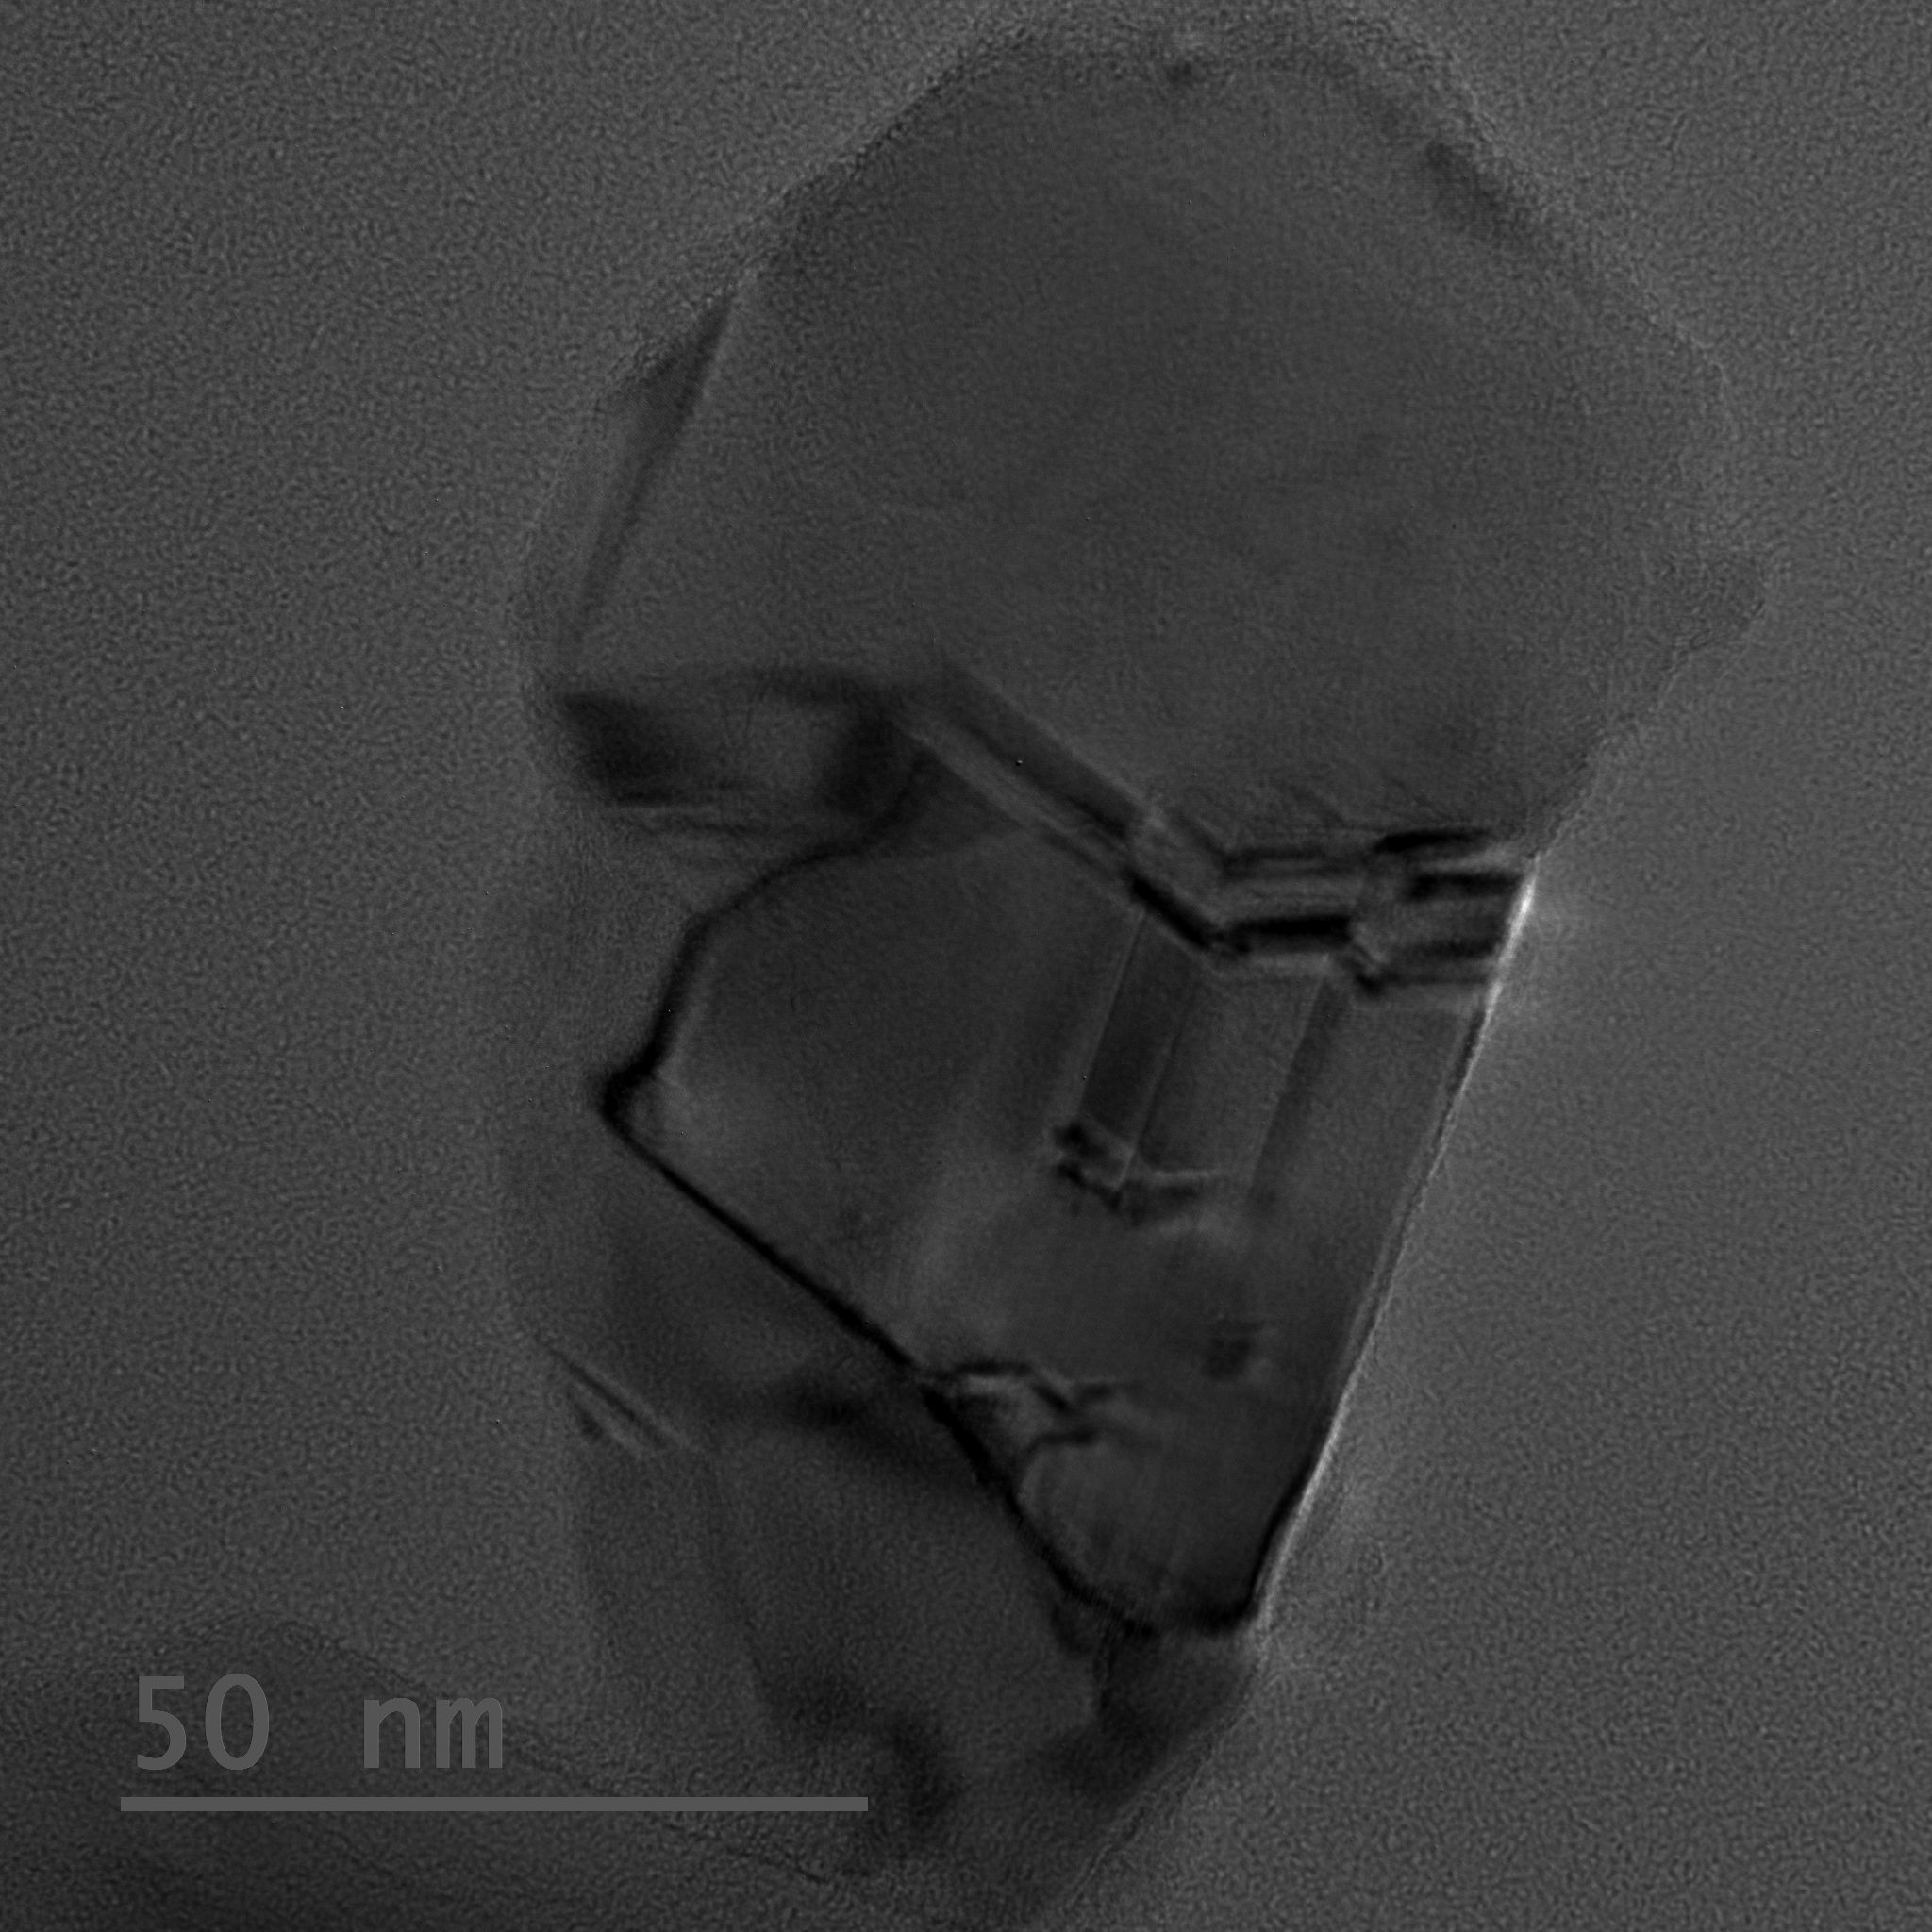
\includegraphics[trim = 0 0 0 0,  clip= true, width = \textwidth]{./pics/AM060-II-k4-2.png}}
					\label{subfig::tem_crystal}
				\end{subfigure}
				\hfill
				\begin{subfigure}[t]{ 0.49\linewidth}
					\centering
					\caption{}
					\testbox{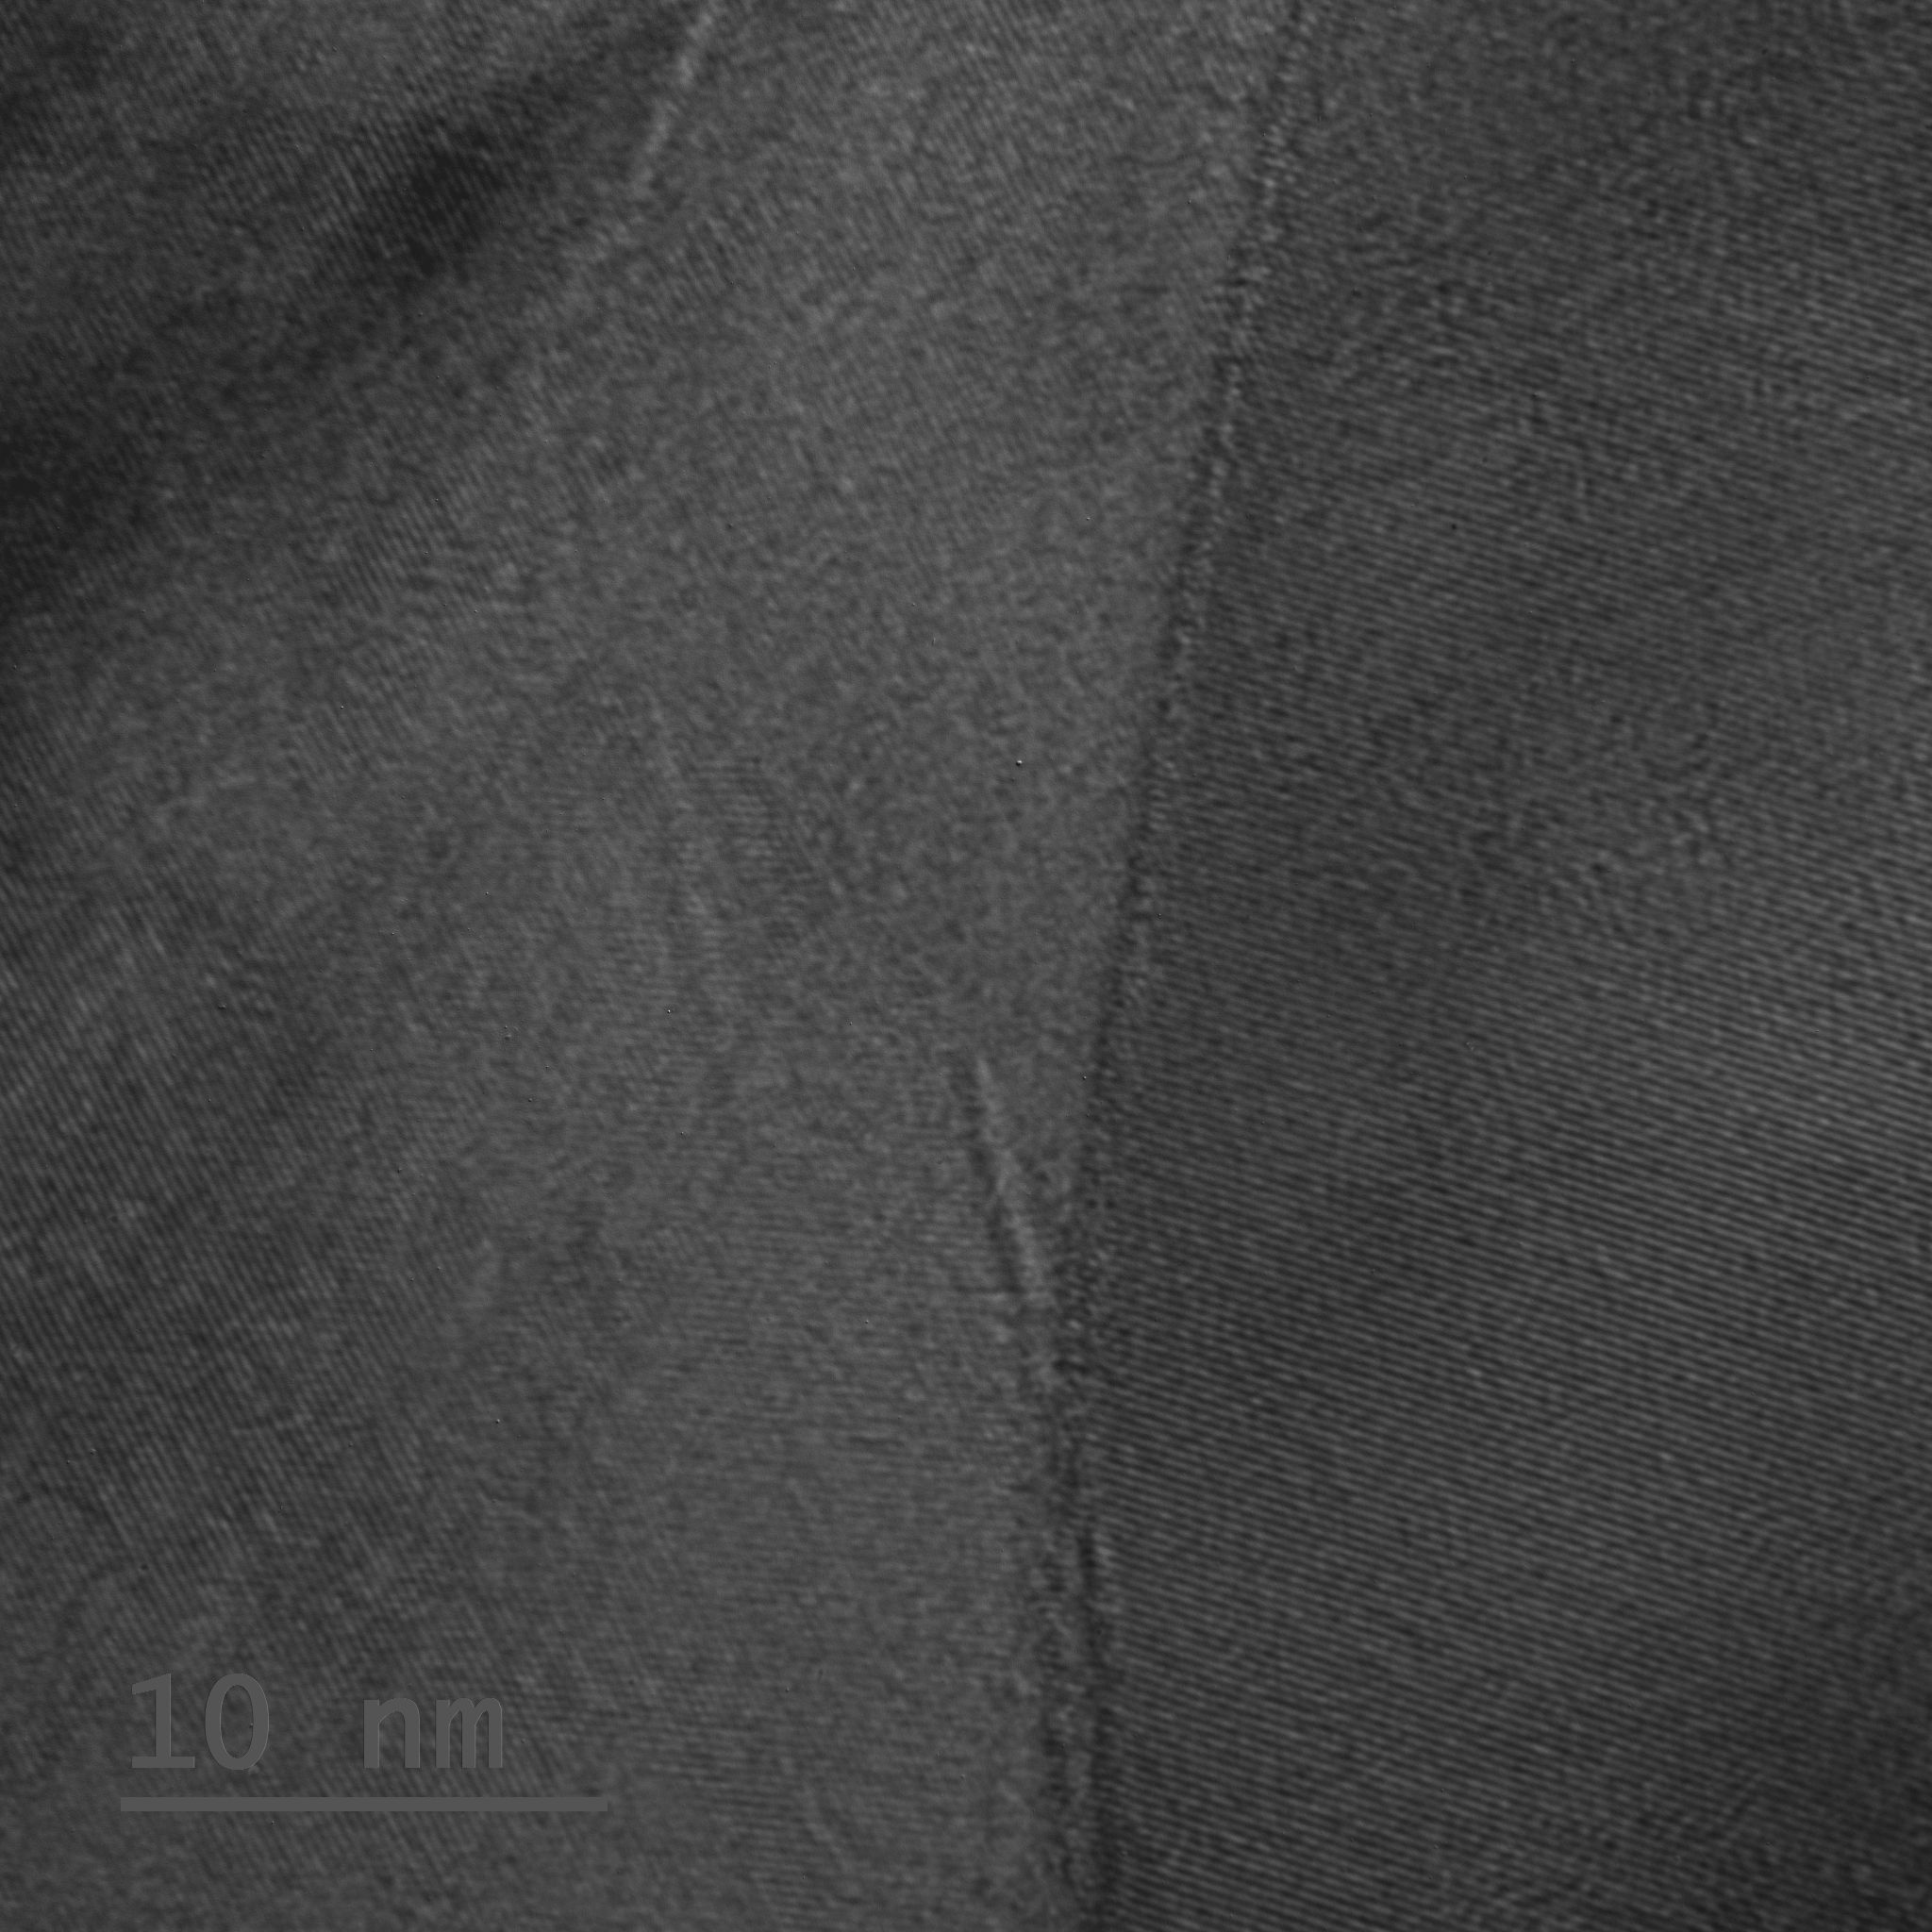
\includegraphics[trim = 0 0 0 0,  clip= true, width = \textwidth]{./pics/AM060-II-k1-3.png}}
					\label{subfig::tem_boundary}
				\end{subfigure}
				\caption[\TEM imaging of a single \nd]{Transmission electron microscopy (TEM) pictures of sample \insituH. (a) Image of a single \nd particle. Several crystal boundaries can be seen within the diamond particle. (b) Close-up image a diamond particle. The vertical line is a crystal boundary, to the left and right the more or less horizontal layers of one crystalline region can be seen.}
				\label{fig::tem}
			\end{figure}

			Transmission electron microscopy (\TEM, also sometimes conventional transmission electron microscopy or CTEM) is a microscopy technique in which a beam of electrons is transmitted through a specimen to form an image. The specimen is most often an ultrathin section less than \SI{100}{\nm} thick or a suspension on a grid. An image is formed from the interaction of the electrons with the sample as the beam is transmitted through the specimen.
			During \tem a beam of electrons is transmitted through a sample, forming an image of the transmitted sample.
			Since electrons have higher de Broglie wavelengths than photons, a higher resolution is obtainable, allowing the surface of \nds to be resolved. Thus, the crystallinity of single \nds can be studied directly.

			\subsection{Crystallinity and Grain Boundaries}\label{subsection::tem_crystal}

				Sample \insituH was investigated using \TEM by \schmauch.
				Smaller \nds would have been too small for the carbon grid which severs as a sample holder in the \TEM, and might have fallen through the grid and bigger bigger particles would have been too big to be transmitted by the electron beam, making the imaging impossible.
				In \autoref{fig::tem} there are \TEM images, one of them exhibits a single diamond particle and the other is a close-up image of a crystal boundary.
				From \autoref{subfig::tem_crystal} it can be seen that the diamond particle contains several crystallites and crystal boundaries.
				The edges of the cristallites are the sharp features within the diamond particle, the crystal boundaries the smoother features\todo{eher nur vermutung}.
				In \autoref{subfig::tem_boundary} the crystal layers which are more or less horizontal and in more or less the middle of the picture there is a vertical line which is the edge of a crystallite.
				So it is clear that the investigated sample does not contain beautiful single crystal diamond particles, which means a reduction of the crystal quality of the diamond particles.
